\documentclass[main.tex]{subfiles}
\begin{document}
\section{Implementation}
All code is available on GitHub \href{https://github.com/DNedilko/CausalDiscoveryProject/tree/244b50fed45bf1547cf7d0a1053891f276ac663b/Project}{DNedilko/CausalDiscovery}. The main language of implementation is Python. 
\subsection{Causal Discovery Setup}
The workflow of the Python code begins with data preparation. The \textt{data\_loader} function ingests a specified subset of columns from a large dataset (HBSC) and has the option to stratify by sex. This data is then cleaned using the \textt{data\_prep} function, which removes rows with missing values according to the specifications outlined in Section \ref{sec:data} and converts the data into a numeric format suitable for subsequent analysis. Textual categorical values are label-encoded, and the DataFrame is transformed into a NumPy array. This ensures that the resulting matrix meets the requirements of the libraries being used.

After data preparation, the pipeline executes the FCI algorithm. The \textt{run\_fci} function applies FCI from \texttt{causal-inference} package to the cleaned data, utilising $G^2$ and $\chi^2$ as the conditional independence test at a specified significance level. The output is a Partial Ancestral Graph (PAG) that encodes the inferred causal relationships among variables. This graph is then visualised and saved as a PNG image. To facilitate a comprehensive analysis, the \texttt{iterator\_over\_fci} function performs parallel execution of FCI across multiple conditional independence tests and significance levels.

\subsection{Parameter Choices}
CI tests $G^2$ and $\chi^2$ are asymptotically similar, so in the interest of time, we have run an experiment to see which CI test would perform better time-wise. We have found that for the particular data, $\chi^2$ CI tests are less effective at scaling. It could be tied to the fact that $G^2$ handles zeroes more optimally and performs logarithmic operations.
\begin{figure}[htbp]
    \centering
    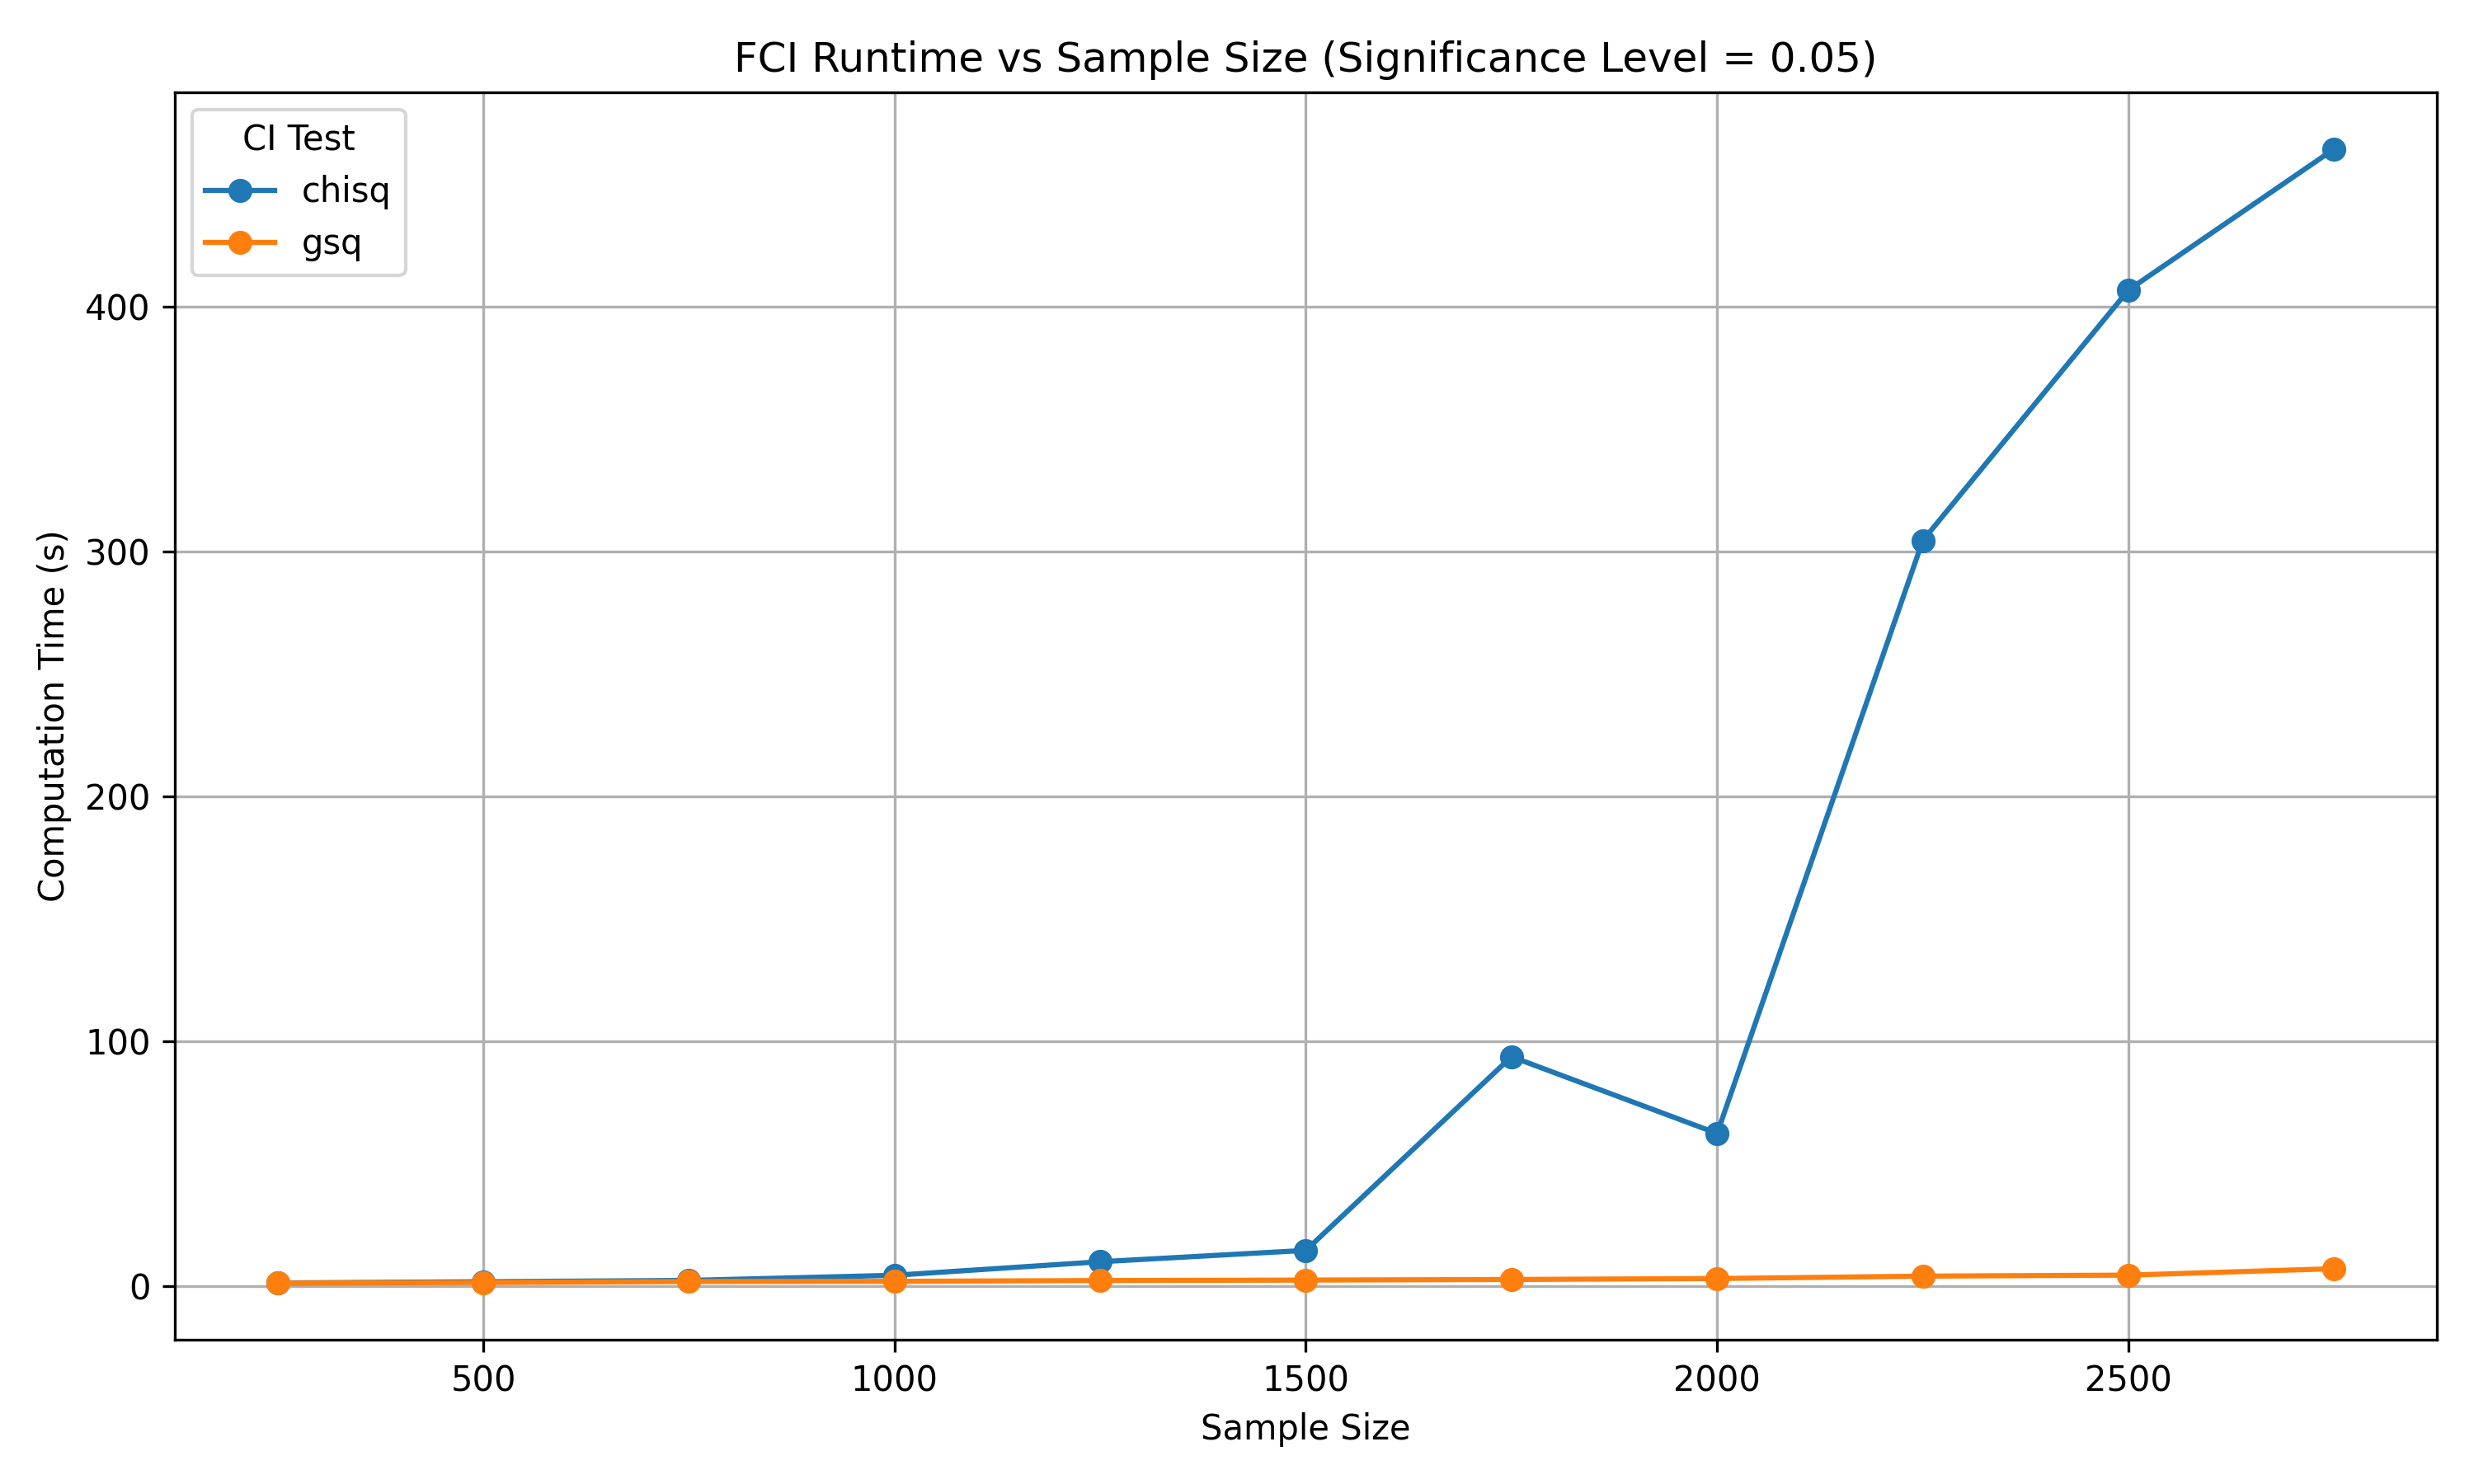
\includegraphics[width=0.8\textwidth]{Report/final_report/pictures/fci_runtime_vs_samplesize.png}
    \caption{Computation time of the FCI algorithm as a function of sample size for different CI tests. The significance level ? is fixed at 0.05 to isolate the effect of increasing data volume on performance.}
    \label{fig:fci_runtime_vs_samplesize}
\end{figure}

\begin{figure}[htbp]
    \centering
    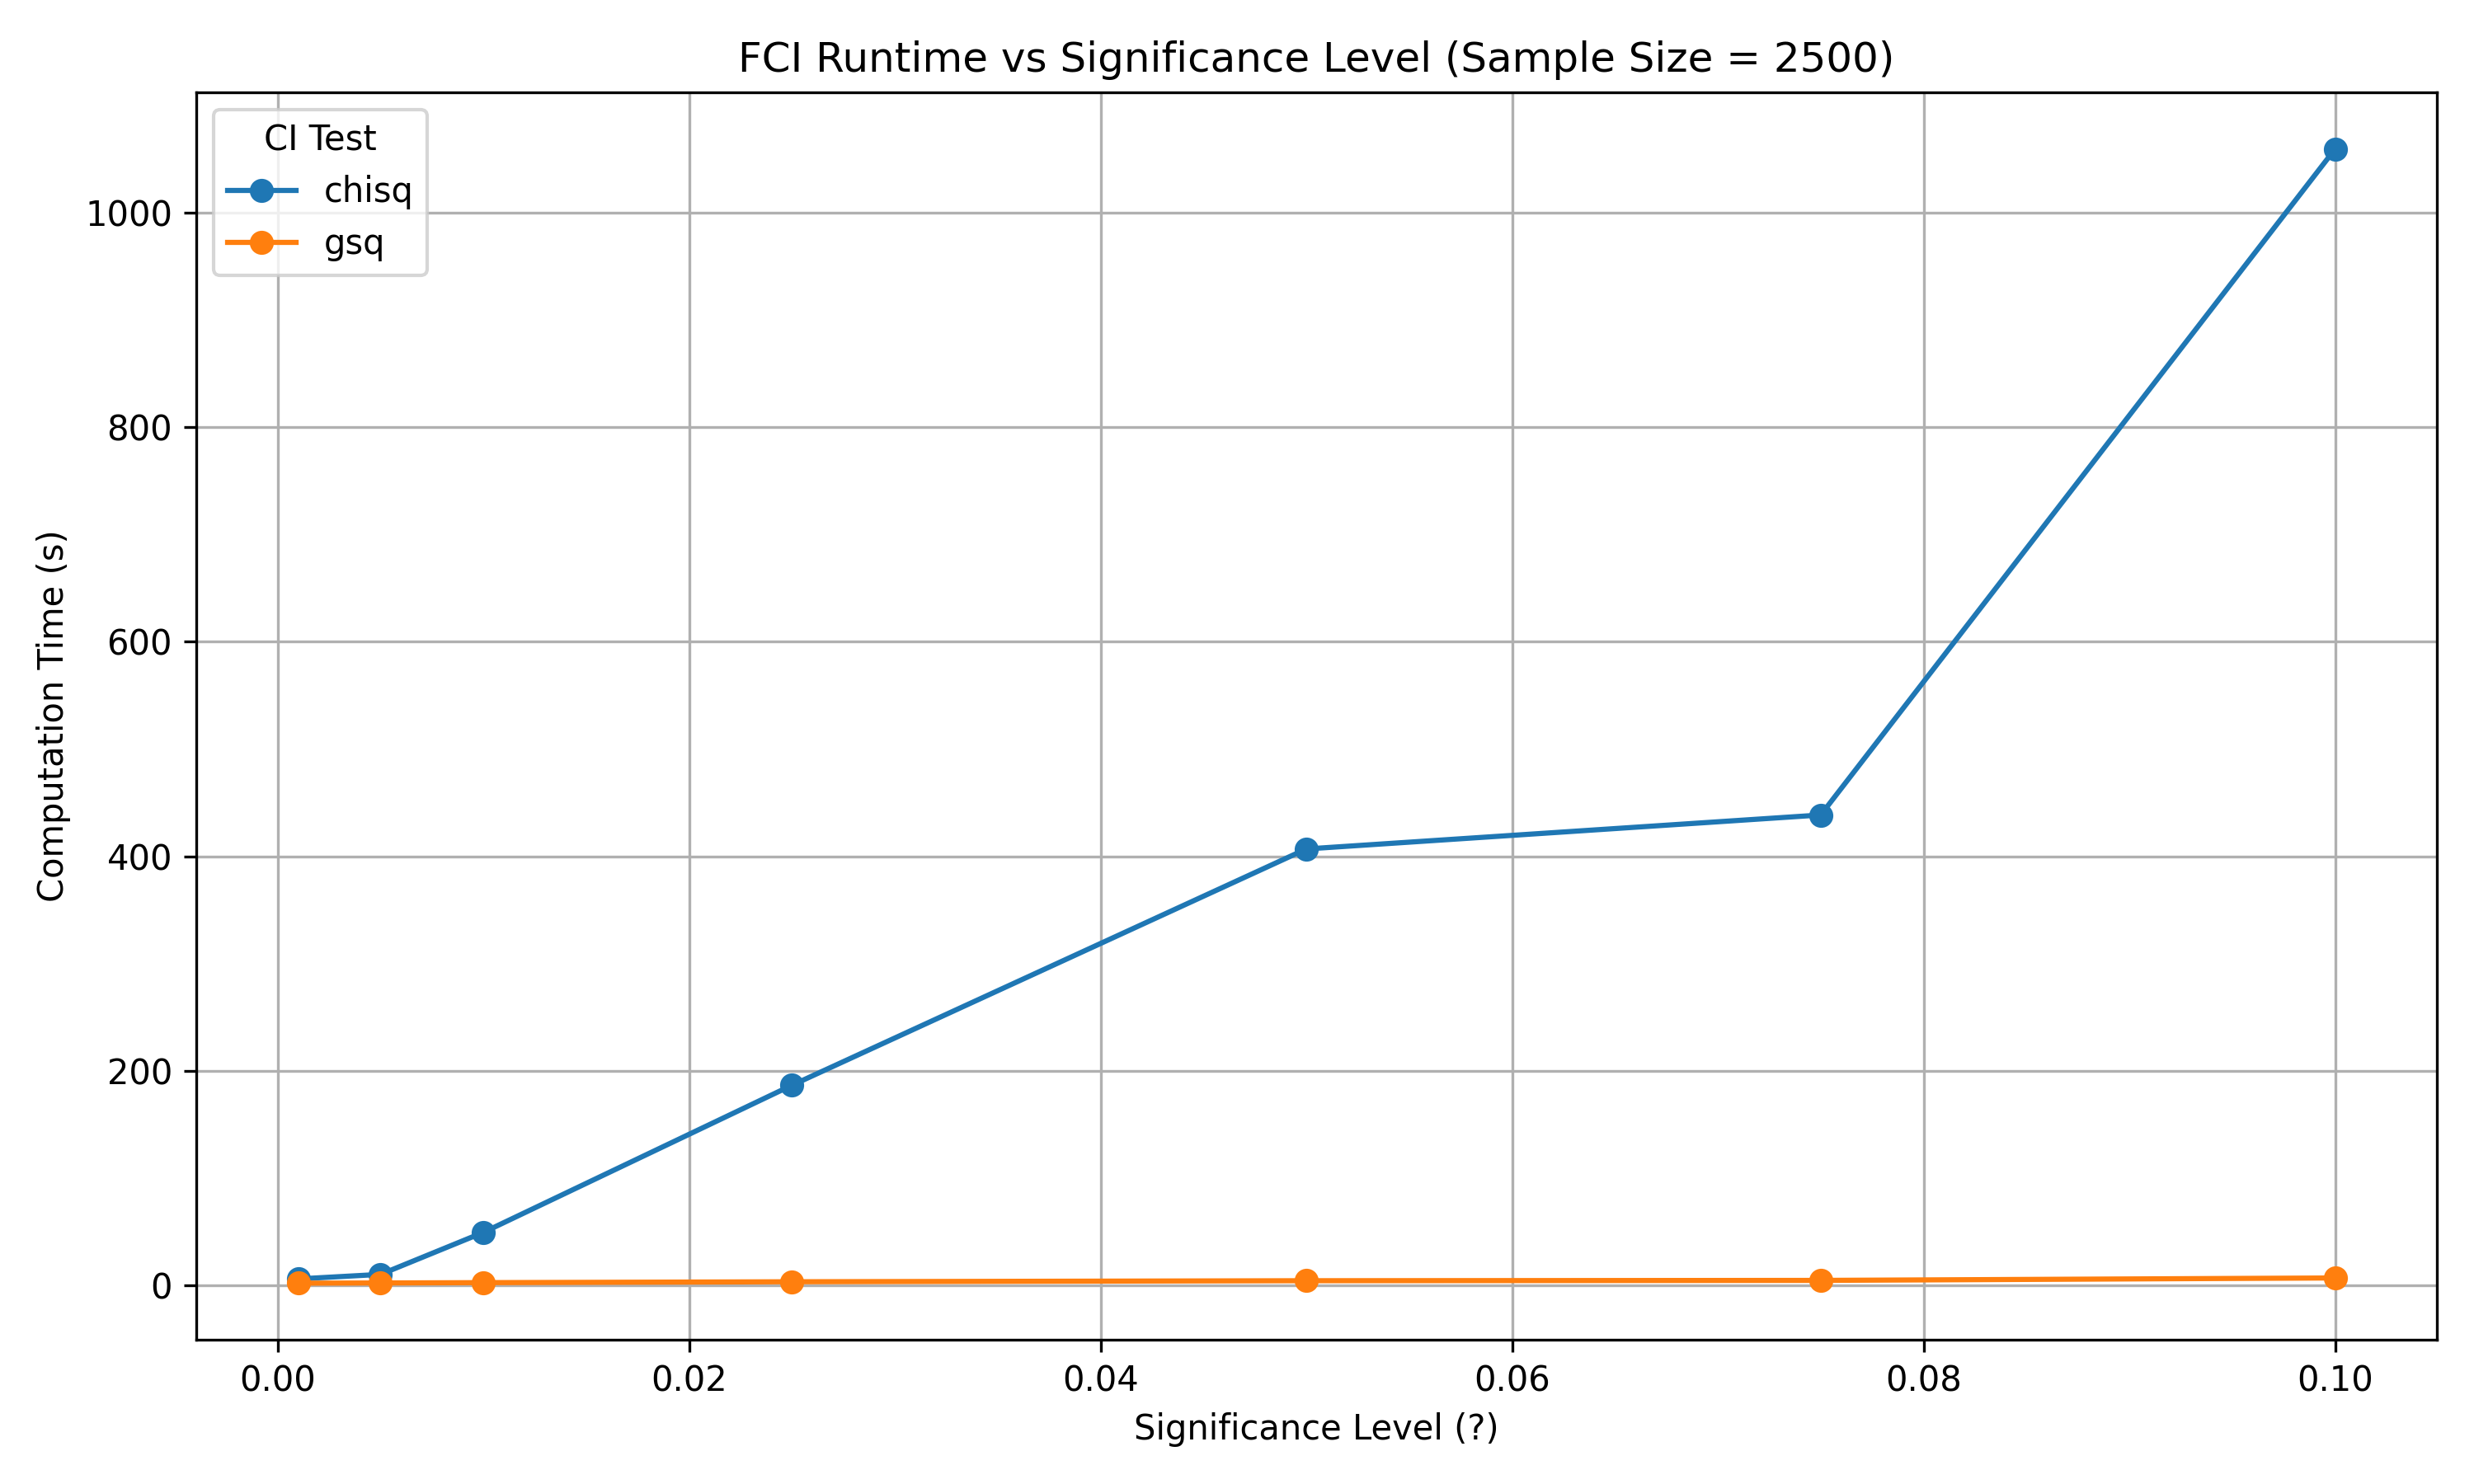
\includegraphics[width=1\textwidth]{Report/final_report/pictures/fci_runtime_vs_alpha.png}
    \caption{Computation time of the FCI algorithm across different significance levels $\alpha$ for various conditional independence (CI) tests. Results are based on a fixed sample size of 2500 observations.}
    \label{fig:fci_runtime_vs_alpha}
\end{figure}



\subsection{Software and Implementation}
In this report, we used the causal-learn library for Python to perform causal discovery on observational data. Example of use:
\small \begin{lstlisting}[language=Python,]
import numpy as np
import pandas as pd
from causallearn.search.ConstraintBased.FCI import fci
from causallearn.utils.cit import  gsq
from causallearn.utils.GraphUtils import GraphUtils


def run_fci(
    data: pd.DataFrame,
    test: = "gsq",
    alpha: float = 0.05) -> tuple:
    
    data_array = data.values.astype(np.float32)

    # Run FCI with specified parameters
    graph, edges = fci(
        dataset=data_array,
        independence_test_method=test,
        alpha=alpha,
        verbose=True
    )

    # Generate a graph visualization
    GraphUtils.to_pydot(graph, labels=data.columns.tolist())
            .write_png(
                os.path.join(output_dir, filename)            )
    return graph, edges

    run_fci(data, test = gsq, alpha = 0.05)
\end{lstlisting}
\subsubsection{\texttt{causal-learn} FCI implementation}
 \texttt{causal-learn} library follows the algorithm in section \ref{sec:methodology}. Besides that, it allows for background knowledge. This function allows to restrict conditional independence  The main \texttt{fci()} function orchestrates the full process. 

\end{document}
